\section{Motivating Example}\label{motivExample}

In this article we discuss context-free constrained path querying, and one of well-known not regular but context-free language is an 
language $$\mathcal{L} = \{A^n B^n; n \geq 1\} = \{AB; AABB; AAABBB; \dots\}$$.
This language is a subset of balanced brackets language and in practice may be used to describe many different relations: n-th generation in parent-child, correct order of an open-close operations for resources, etc.

Let consider the graph $M=(\{0;1;2;3\},E,\{A;B\})$ is presented in figure~\ref{input} which labels represent one of mentioned relations.
We want to find all paths $p$, such that $\Omega(p) \in \{AB; AABB; AAABBB; \dots\}$ or $\Omega(p) \in A^n B^n$ where $n \geq 1$.
Required language can be specified by grammar $G_1$ presented in picture~\ref{grammarG} where $N = \{s; middle\}$, $\Sigma = \{A; B\}$, and $S = s$.

\begin{figure}[h]
    \begin{center}
        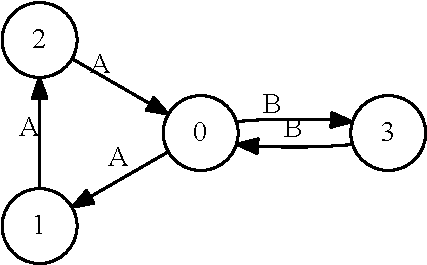
\includegraphics[width=6cm]{dot/input.pdf}
        \caption{Input graph $M$}
        \label{input}        
    \end{center}
\end{figure}

\begin{figure}[h]
   \begin{center}
\begin{verbatim}
   0: s = A s B 
   1: s = middle
   2: middle = A B
\end{verbatim}
   \caption{Grammar $G_1$ for language $L=\{A^n B^n; n \geq 1\}$}
   \label{grammarG}        
   \end{center}
\end{figure}

Result of presented query for given graph is an infinite set of paths, hence it cannot be constructed explicitly. 
Moreover, for some tasks it can be necessary to get the structure of result with respect to given grammar.
Further we show how to get finite representation of query result structure in terms of derivation in grammar.
